\section{Dynamics of the Ising model}

\subsection{Purpose of the Glauber dynamic}

The Ising model is a correlated model, meaning that the spins are not independent
(except, of course, when $\beta=0$).
A broad strategy for analysing correlated models is by somehow decomposing them into independent pieces.
It is often difficult to implement such a scheme, and strategies vary wildly between models.

In this section, we describe how the Ising model is the unique stationary distribution
of a certain Markov chain, called the \emph{Glauber dynamic}.
This Markov chain can be sampled using independent randomness at each step,
which gives a decomposition of the Ising model into independent pieces.
On the one hand, Glauber dynamics are useful because it gives a simple
way to \emph{simulate} the Ising model (take approximate samples from it using a computer).
The Glauber dynamic is closely related to the \emph{Metropolis--Hastings algorithm},
and belongs to a class of \emph{Markov Chain Monte Carlo} (MCMC) algorithms.
On the other hand, we can analyse this Markov chain to rigorously prove
a number of theoretical results about the Ising model.

\subsection{Definition of the Glauber dynamic}

\begin{figure}
    \centering
    \includegraphics{figures/glauber.pdf}
    \caption{The Glauber dynamic randomly selects a vertex,
    as well as a uniform random variable $\iota\in[0,1]$.
    If $\iota$ is below the threshold value, then the chosen spin is set to $-1$;
    if it is above, the spin is set to $+1$.
    The threshold value is chosen in such a way that the Markov chain mixes to the desired distribution on $\Omega$.}
    \label{fig:glauber}
\end{figure}

The idea of the Glauber dynamic is simple: at each step, we pick a vertex $u\in V$ uniformly at random,
erase the value of $\sigma_u$,
and then sample the value of $\sigma_u$ from the conditional measure $\mu[\blank|(\sigma_v)_{v\neq u}]$
(see Figure~\ref{fig:glauber}).

We first define a probability measure $\P$ that serves as a source of independent randomness for this Markov chain.

\begin{definition}[Auxilliary randomness on finite graphs]
    Let $G=(V,E)$ denote a finite simple graph.
    Let $(u_i,\iota_i)_{i\geq 1}$ be an i.i.d.~sequence of random variables,
    such that the law of $(u_i,\iota_i)$ is uniform in $V\times[0,1]$.
    Write $\P$ for the associated probability measure.
\end{definition}

Let us now describe how this randomness can be used to update a state $\sigma\in\Omega=\{\pm1\}^V$.

\begin{definition}[Update map]
    \label{def:Update map}
    Let $\mu$ denote a probability measure on $\Omega$,
    and let $\sigma$ denote a state in the support of $\mu$.
    For each pair $(u,\iota)\in V\times[0,1]$, we define
    \begin{equation}
        \label{eq:Update map}
    R_{u,\iota}^\mu(\sigma):=
    \begin{cases}
        f_u^-(\sigma) & \text{if $\iota\leq\mu[\{\sigma_u=-1\}|(\sigma_v)_{v\neq u}]$},\\
        f_u^+(\sigma) & \text{otherwise},
    \end{cases}
    \end{equation}
    where \[
    f_u^\pm:\Omega\to\Omega,\,
    \sigma\mapsto
    \text{the state $\sigma$, except that $\sigma_u$ is set to $\pm1$}.
    \]
\end{definition}

\begin{definition}[Glauber dynamic]
    Let $G=(V,E)$ be a finite simple graph.
    Let $\mu$ denote a probability measure on $\Omega$,
    and $\sigma$ a state in the support of $\mu$.
    The \emph{Glauber dynamic} is the Markov chain $X=X^\mu=(X^\mu_k)_{k\in\Z_{\geq 0}}$ defined via
    $X^{\mu}_0=\sigma$ and
    \[
        X^{\mu}_{k+1}:=R_{u_{k+1},\iota_{k+1}}^\mu(X^{\mu}_k).
    \]
    The dependency on $\sigma$ is implicit, and the reference to $\mu$ is sometimes omitted.
\end{definition}

We are now going to prove that the Markov chain $X^\mu$ mixes to $\mu$.

\begin{lemma}[Convergence of the Glauber dynamic]
    Let $G$ denote a finite simple graph,
    and $\P$ the associated auxilliary randomness probability measure.
    Let $\mu$ denote any probability measure on $\Omega$.
    If the Markov chain $X^\mu$ is irreducible,
    then for any starting state $\sigma$ in the support of $\mu$,
    the distribution of $X^\mu_k$ converges to $\mu$ as $k\to\infty$.
\end{lemma}

\begin{proof}
    \textbf{Aperiodicity.}
    The Markov chain is aperiodic because the probability of staying in the same state is positive.
    \textbf{Convergence.}
    Since the Markov chain is irreducible and aperiodic,
    it suffices to show that $\mu$ satisfies the detailed balance equation
    for the matrix of transition probabilities of $X^\mu$.
    Since the Markov chain can only transition between states that differ at a single vertex,
    it suffices to check the detailed balance equation such a pair of states.
    Let $\sigma^-,\sigma^+\in\Omega$ be two states that differ at exactly one vertex $v\in V$,
    where $\sigma^-_v=-1$ and $\sigma^+_v=+1$.
    Let $Q$ denote the event that some spin configuration equals $\sigma^-$ on $V\setminus\{v\}$.
    Then
    \begin{align}
        \mu[\sigma^-]
        \cdot
        \P[\{X^\mu_{1}=\sigma^+\}|\{X^\mu_0=\sigma^-\}]
        &=\mu[\sigma^-]\cdot\P[\{R_{u_1,\iota_1}^\mu(\sigma^-)=\sigma^+\}]
        \\&=
        \mu[\sigma^-|Q]\mu[Q]\cdot\frac1{|V|}
        \P\Big[\Big\{\iota_1 > \mu[\sigma^-|Q]\Big\}\Big]
        \\&=
        \mu[\sigma^-|Q]\mu[Q]\cdot\frac1{|V|}\mu[\sigma^+|Q].
    \end{align}
    We can also work out $\mu[\sigma^+]\cdot\P[\{X^\mu_{1}=\sigma^-\}|\{X^\mu_0=\sigma^+\}]$,
    which yields the same expression (that is symmetric in $\sigma^-$ and $\sigma^+$).
    This proves the detailed balance equation.
\end{proof}

\begin{remark}
    Consider the Ising model $\mu_{G,\beta}$ on a finite simple graph $G=(V,E)$ at inverse temperature $\beta\in[0,\infty)$.
    It is then easy to see that every state has a positive probability of ocurring.
    The Glauber dynamic can therefore flip any spin at each step.
    It can thus hop from one state to any other state in at most $|V|$
    steps, proving irreducibility.
    The Markov chain is very easy to implement in a computer,
    and has been used by theoretical physicists to simulate the Ising model
    in order to make meaningfull predictions.
\end{remark}

\begin{lemma}[Glauber update for conditioned measures]
    Consider a finite simple graph $G=(V,E)$.
    Consider a probability measure $\mu$ on $\Omega$ such that every state has a positive probability.
    For $\Lambda\subset V$ and $\zeta\in\{\pm1\}^{V\setminus\Lambda}$,
    define the measure $\nu:=\mu[\blank|\{\sigma|_{\Lambda^\complement}=\zeta\}]$.
    Then:
    \begin{itemize}
        \item For $u\in\Lambda$, we have $R_{u,\iota}^\nu=R_{u,\iota}^\mu$ (at least on the support of $\nu$),
        \item For $u\in\Lambda^\complement$, we have $R_{u,\iota}^\nu=f_u^{\zeta_u}$ (at least on the support of $\nu$).
    \end{itemize}

    Moreover,
    \begin{itemize}
        \item We may extend $R_{u,\iota}^\nu$ from $\operatorname{Support}(\nu)$ to $\Omega$ via the equalities above,
        % \item These extensions are still monotone,
        \item The associated Markov chain in $\P$ is irreducible and mixes to $\nu$.
    \end{itemize}
\end{lemma}

\begin{proof}
    This follows straightforwardly from the definitions.
    Remark that the Markov chain is irreducible and mixes to $\nu$:
    almost surely, all vertices in $V\setminus\Lambda$ are given the correct spin at some point,
    and the support of $\nu$ is connected by single sign flips.
\end{proof}


\subsection{Ferromagnetism in the Ising model}

\begin{theorem}[Ferromagnetism]
    \label{thm:Ferromagnetism}
    Fix a finite simple graph $G$ and a constant $\beta\in[0,\infty)$.
    Consider a fixed vertex $u$.
    Let $N_+(\sigma)$ denote the number of neighbours of $u$
    at which $\sigma$ takes the value $+1$,
    and $N_-(\sigma)$ the number of neighbours with value $-1$.
    Write $(N_+(\sigma)-N_-(\sigma)):=N_+(\sigma)-N_-(\sigma)$.
    Then
    \begin{equation}
        \label{eq:Ferromagnetism}
        \mu_{G,\beta}[\{\sigma_u=+1\}|(\sigma_v)_{v\neq u}]
        =
        \frac{e^{\beta (N_+(\sigma)-N_-(\sigma))}}{2\cosh (\beta (N_+(\sigma)-N_-(\sigma)))}.
    \end{equation}
    This function is increasing in $(N_+(\sigma)-N_-(\sigma))$, which is increasing in $\sigma$.

    \textbf{In other words, the more spins around $u$ are valued $+$,
    the more likely it is that $\sigma_u=+$. This property is called \emph{ferromagnetism}
    and it is an essential feature of the Ising model.}
\end{theorem}

\begin{proof}
    If all spins except for the spin $\sigma_u$ are known,
    then the likelyhood of the remaining spin $\sigma_u$ is proportional to $e^{\beta(N_+(\sigma)-N_-(\sigma))\sigma_u}$.
    The formula in the theorem then follows.
\end{proof}

For the avoidance of doubt, let us define what we mean by an \emph{increasing function}.

\begin{definition}[$\Omega$ as a partially ordered set]
    Let $G$ denote a simple graph.
    We introduce a partial order $\leq$ on $\Omega$ such that
    $\sigma\leq\tau$ if and only if $\sigma_v\leq\tau_v$ for all $v\in V$.

    Let $\calA$ and $\calB$ denote two arbitrary partially ordered sets.
    We say that a function $f:\calA\to\calB$ is \emph{increasing} if $\sigma\leq\tau$ implies $f(\sigma)\leq f(\tau)$ for all $\sigma,\tau\in\calA$.
    Such a  function is called \emph{decreasing} if $\sigma\leq\tau$ implies $f(\sigma)\geq f(\tau)$ for all $\sigma,\tau\in\calA$.
\end{definition}

\begin{figure}
    \centering
    \includegraphics{figures/mono.pdf}
    \caption{Ferromagnetism of the Ising model implies that applying the Glauber update
    with the external source of randomness $(u,\iota)$ preserves the ordering of the configurations.}
    \label{fig:mono}
\end{figure}

The monotonicity property in the previous theorem has profound implications,
that we will come back to very soon.
We shall first study the Glauber dynamic at very high temperature ($\beta\approx0$).
In that case, Equation~\eqref{eq:Ferromagnetism} tells us that the threshold value is very close to $1/2$.

\subsection{High-temperature Glauber dynamic}

Ising proved that the 1D model does not undergo a phase transition (it has exponential decay at all temperatures),
and Peierls proved that the 2D model does have a magnetised phase.
We did not yet prove that the 2D model undergoes a phase transition;
it could be magnetised at all temperatures.
We shall now prove that this is not the case: we prove that it also exhibits exponential decay at high temperatures.
This holds true for any graph with a bounded degree.

There are \emph{many} ways to prove this fact.
Here we use the dependency structure of the Glauber dynamic, which is easy to analyse at high temperatures.
It recycles an energy vs.\ entropy calculation we saw before in the Peierls argument.

\begin{figure}
    \centering
    \includegraphics{figures/dependency.pdf}
    \caption{The set $\bar\Lambda\times\Z_{\geq 0}$.
    On the left, we see the dependency structure of the Glauber dynamic.
    On the right, we see the same structure,
    but with the edges emenating from ``good'' Glauber updates (in green) removed.
    The idea is that when $\beta$ is very small, then most of the Glauber updates are ``good''.
    In that case, the dependency tree of each vertex is typically very small, and in particular it is exponentially unlikely
    to reach $\partial\Lambda$ or the initial condition.}
    \label{fig:dependency}
\end{figure}

\begin{definition}[Dependency structure, Figure~\ref{fig:dependency}]
    Consider the Glauber dynamic on the Ising model $\mu:=\langle\blank\rangle_{\Lambda,\beta}^\zeta$
    where $\Lambda$ is a finite vertex subset of some locally finite graph $G$,
    and $\zeta$ a boundary condition.
    Recall that the auxilliary measure $\P$ is the law of the i.i.d.~sequence $(u_i,\iota_i)_{i\geq 1}$,
    where $(u_i,\iota_i)$ is uniform in $\bar\Lambda\times[0,1]$.

    Let $\calD=\calD((u_i)_i)$ be the \emph{dependency graph} of the Glauber dynamic, defined as the following directed graph:
    \begin{itemize}
        \item Its vertices $V(\calD)\subset\bar\Lambda\times\Z_{\geq 0}$ are given by
        \begin{equation}
            V(\calD):=(\bar\Lambda\times\{0\})\;\cup\;(\partial\Lambda\times\Z_{\geq 0})\;\cup\;\{(u_i,i):i\in\Z_{> 0}\},
        \end{equation}
        \item Its directed edges $E(\calD)$ are given by
        \begin{equation}
            E(\calD):=\{((u,i),(v,j))\in V(\calD)^2:\text{$u\in\Lambda$, $v\sim u$, and $j=\max\{j'<i:(v,j')\in V(\calD)$}\}\}.
        \end{equation}
    \end{itemize}
    We shall also write $\partial\calD:=(\bar\Lambda\times\{0\})\cup(\partial\Lambda\times\Z_{\geq 0})$.
    Notice that $\calD$ is a random directed graph in $\P$
    that is measurable in terms of $(u_i)_i$.
\end{definition}

\begin{lemma}
    Consider the Glauber dynamic on the Ising model $\mu:=\langle\blank\rangle_{\Lambda,\beta}^\zeta$
    where $\Lambda$ is a finite vertex subset of some locally finite graph $G$,
    and $\zeta$ a boundary condition.

    Fix $v\in\Lambda$ and $T\in\Z_{\geq 0}$.
    Let $i\leq T$ denote the largest index such that $(v,i)\in V(\calD)$.
    Then the value of $X_T(v)$ is measurable in terms of:
    \begin{itemize}
        \item The set $\calC^{v,T}$ of $\calD$-vertices reachable from $(v,i)$ by following \emph{outgoing} $\calD$-edges,
        \item The values of the initial/boundary conditions on $\calC^{v,T}\cap\partial\calD$,
        \item The values of $\iota$ on $\calC^{v,T}\setminus\partial\calD$.
    \end{itemize} 
\end{lemma}

\begin{proof}
    This follows by definition of the Glauber dynamic and the dependency structure.
\end{proof}

Suppose that $G=(V,E)$ is a simple graph whose max-degree is $K\in\Z_{\geq 0}$.
Then the expression in Equation~\eqref{eq:Ferromagnetism} lies in the interval
\begin{equation}
    \label{eq:constrained_interval}
    [\tfrac12 - \tfrac12 \tanh (\beta K),\tfrac12 + \tfrac12 \tanh (\beta K)]=: I_{K,\beta}\subset [0,1].
\end{equation}
Now go back to the Glauber dynamic in the context of the Ising model.
If $\iota\not\in I_{K,\beta}$,
then we see from Equation~\eqref{eq:Update map} that the update map $R_{u,\iota}^{\mu_{G,\beta}}$
does not actually care about $\sigma$ when deciding to set $\sigma_u$ to $+1$ or $-1$.
More precisely, we have
\[
    R_{u,\iota}^{\mu_{G,\beta}}(\sigma)
    =
    \begin{cases}
        f_u^-(\sigma) & \text{if $\iota < \tfrac12 - \tfrac12 \tanh (\beta K)$,} \\
        f_u^+(\sigma) & \text{if $\iota > \tfrac12 + \tfrac12 \tanh (\beta K)$,} \\
        f_u^{\text{``something depending on $\iota$ and $N_+(\sigma)-N_-(\sigma)$''}}(\sigma) & \text{if $\iota\in I_{K,\beta}$.}
    \end{cases}
\]
Thus, with probability $1-\tanh(\beta K)$,
we have $\{\iota\not\in I_{K,\beta}\}$.
This means that we do not need to inspect $\sigma$ before determining the new value of $\sigma_u$.
With probability $\tanh(\beta K)$, we have $\{\iota\not\in I_{K,\beta}\}$,
and the new value for $\sigma_u$ actually depends on the ``old'' values of $\sigma$
at the neighbours of $u$.

\begin{theorem}[Exponential decay at high temperature]
    Let $G=(V,E)$ be a simple graph of maximum degree $K\in\Z_{\geq 0}$,
    and fix $v\in V$.
    Fix $\beta\in[0,\infty)$.
    Let $\Lambda_n$ denote the set of vertices at a graph distance smaller than $n$ from $v$.
    Then if $K\tanh(\beta K)<1$, the magnetisation of $\sigma_v$ vanishes exponentially fast in the distance to the boundary,
    in the sense that for all $n$ we have
    \[
        |\langle\sigma_v\rangle_{\Lambda_n,\beta}^+| \leq \frac{(K\tanh(\beta K))^n}{1-K\tanh(\beta K)}.
    \]
    This theorem applies in particular to the setup of Theorem~\ref{thm:peierls}.
\end{theorem}

\begin{proof}
    For fixed $n$, write $\P_n$ and $\calD_n$ for the associated auxilliary randomness measure and dependency structure.
    Call a $\calD_n$-vertex $(u,i)$ \emph{good} if $\iota_i\not\in I_{K,\beta}$
    and \emph{bad} otherwise.
    Fix $T\in\Z_{\geq 0}$.
    Notice that:
    \begin{itemize}
        \item Conditional on $\calC^{v,T}_n$, each vertex in $\calC^{v,T}_n\setminus\partial\calD_n$ is bad with probability $\tanh(\beta K)$,
        independently of the state of the other vertices,
        \item If we furthermore condition on the event that $\calC^{v,T}_n$ does \emph{not} contain a path towards $\partial\calD_n$
        consisting of only bad $\calD_n$-vertices, then the conditional law of $X_{n,T}(v)$ is that of a fair coin flip.
    \end{itemize}
    It suffices to prove the second inequality in the following equation:
    \begin{equation}
        |\langle\sigma_v\rangle_{\Lambda_n,\beta}^+| \leq\lim_{T\to\infty}
        \P_n[\{\text{there exists a bad path from $(v,T)$ to $\partial\calD_n$}\}]
        \leq
        \frac{(K\tanh(\beta K))^n}{1-K\tanh(\beta K)}.
    \end{equation}
    First of all, it is easy to see that the probability that a bad path reaches to the initial condition $\Lambda\times\{0\}$,
    tends to zero with $T$ (in fact, for fixed $n$, it tends to zero exponentially fast in $T$ by standard properties of finite state Markov chains).
    It suffices to prove that
        \begin{equation}
        \lim_{T\to\infty}
        \P_n[\{\text{there exists a bad path from $(v,T)$ to $\partial\Lambda\times\Z_{\geq 0}$}\}]
        \leq
        \frac{(K\tanh(\beta K))^n}{1-K\tanh(\beta K)}.
    \end{equation}
    Now every path from $(v,T)$ to $\partial\Lambda\times\Z_{\geq 0}$ may be associated
    with a unique $\bar\Lambda$-path, by simply forgetting the second coordinate (the time at which the Glauber updates were performed).
    Such paths $\gamma$ satisfy the following criteria:
    \begin{itemize}
        \item They start at $v$,
        \item They end at $\partial\Lambda$, and never visit $\partial\Lambda$ except at the last step,
        \item They may visit the other vertices multiple times.
    \end{itemize}
    Moreover, this ``projection of paths'' is injective when considering paths starting at the same point $(v,T)$.
    Thus, we get
    \begin{align}
        |\langle\sigma_v\rangle_{\Lambda_n,\beta}^+|
        &\leq
        \lim_{T\to\infty}
        \P_n[\{\text{there exists a bad path from $(v,T)$ to $\partial\Lambda\times\Z_{\geq 0}$}\}]
        \\&\leq
        \sum_{\gamma:v\to\partial\Lambda_n}\lim_{T\to\infty} \P_n[\{\text{the path corresponding to $\gamma$ is bad}\}]
        \\&=
        \sum_{\gamma:v\to\partial\Lambda_n} \tanh(\beta K)^{|\gamma|}.
    \end{align}
    Such a path must have a length of at least $n$,
    and there are at most $K^\ell$ paths of length $\ell$.
    Thus, by bounding the last expression in the previous display, we obtain
    \begin{equation}
        |\langle\sigma_v\rangle_{\Lambda_n,\beta}^+|
        \leq
        \sum_{\ell=n}^\infty (K\tanh(\beta K))^\ell
        =  \frac{(K\tanh(\beta K))^n}{1-K\tanh(\beta K)}.
    \end{equation}
    This is the desired exponential decay.
\end{proof}

\begin{exercise}[Exponential decay of correlation functions]
    Consider the square lattice graph $\Z^d$ in dimension $d\in\Z_{\geq 2}$.
    Fix $\beta\in[0,\infty)$ with $2d\tanh(2\beta d)<1$.
    Write $\Lambda_n:=((-n,n)\cap\Z)^d$.

    Now fix a finite subset $A\subset\Lambda_k$ for some fixed $k\in\Z_{\geq 1}$,
    and prove that
    \[
        \textstyle
        |\langle \prod_{v\in A} \sigma_{nv} \rangle_{\Lambda_{nk},\beta}^+|
    \]
    tends to zero exponentially fast in $n$.

    \emph{Hint: start with $|A|=2$, and consider the dependency structure of both points in $A$.}
\end{exercise}





\subsection{Consequences of ferromagnetism}

\begin{lemma}[Monotonicity of the Glauber update, cf.~Figure~\ref{fig:mono}]
    Let $G$ be a finite simple graph, and choose $\beta\in[0,\infty)$.
    Then for any pair $(u,\iota)\in V\times[0,1]$ the map
    \begin{equation}
        \label{eq:Monotonicity of the Glauber update:free}
        R_{u,\iota}^{\mu_{G,\beta}}:\Omega\to\Omega
    \end{equation}
    is an increasing function.
\end{lemma}

\begin{proof}
    Write $\mu:=\mu_{G,\beta}$.
    Recall Definition~\ref{def:Update map} and focus on Equation~\eqref{eq:Monotonicity of the Glauber update:free}.
    Observe that the threshold value $\mu[\{\sigma_u=-1\}|(\sigma_v)_{v\neq u}]$
    is a \emph{decreasing} function of $\sigma$, by ferromagnetism (Theorem~\ref{thm:Ferromagnetism}).
    Since $\sigma_u$ is set to $+1$ when $\iota$ exceeds the threshold value,
    it is easy to see that $R_{u,\iota}^\mu$ is an increasing function of $\sigma$
    for fixed $u$ and $\iota$.
\end{proof}


\begin{lemma}[Monotonicity of the grand coupling]
    Let $G$ denote a finite simple graph and consider $\beta\in[0,\infty)$.
    Consider the 
\end{lemma}

